\chapter{Work Package Tasks}
\label{ch:wptasks}

In this chapter, we discuss in brief about the high level tasks in each WP. A reference architecture diagram is also given for each WP, this is meant to be seen as an early proposal and it is subjected to change in future documents.

\section{WP1: Service Descriptor Translator}

\subsection{Requirements definitions and architecture design}

\begin{figure}[h]
	\centering
	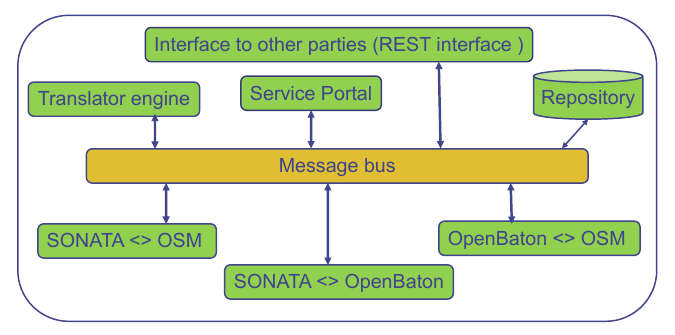
\includegraphics[width=0.9\linewidth]{figures/wp1Arch}
	\caption{Reference architecture for SDT}
	\label{fig:wp1arch}
\end{figure}

\subsection{Prototype implementation of SDT components}
\subsection{Proof of concept demonstration}

\section{WP2: Service Descriptor Splitter}

\subsection{Requirements definition and architecture design}
\paragraph{}
\begin{figure}[h]
	\centering
	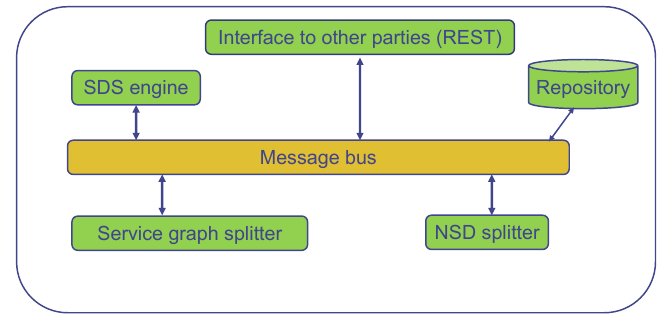
\includegraphics[width=0.9\linewidth]{figures/wp2Arch}
	\caption{Reference architecture for SDS}
	\label{fig:wp2arch}
\end{figure}

\subsection{Investigation of service graph partitioning algorithms and libraries}
\subsection{Prototype implementation of SDS components}
\subsection{Proof of concept demonstration}


\section{WP3: MANO Adaptor}

\subsection{Requirements definition and architecture design}
\paragraph{}

\begin{figure}[h]
	\centering
	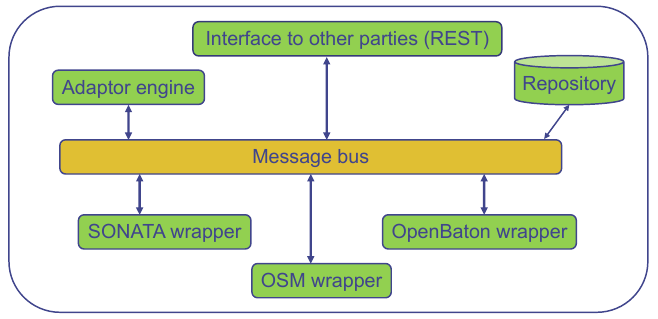
\includegraphics[width=0.9\linewidth]{figures/wp3Arch}
	\caption{Reference architecture for MA}
	\label{fig:wp3arch}
\end{figure}

\subsection{Prototype implementation of adaptor components}
\subsection{Investigation of MANO scalability challenges}
\subsection{Proof of concept demonstration}
